\documentclass[./main]{subfiles} % これを最初に書く


% ここにnewtheorem,newenvironment,defなどを書く
\newtheorem{theo}{定理}
\newtheorem{defi}{定義}
\newtheorem{rem}{注意}

\begin{document} %ここから文章を始める

\Chapter{四次元立方体の描き方()} 
% 章だてはSection,Subsection,Subsubsectionで行う
\Section{四次元立方体を描いてみよう}

四次元の立体がどのような形状をしているのか,ほとんどの方は正確にイメージすることができないと思います.それは我々が手に取って観察できる立体が,三次元より低い次元のものしかないからです.

では,我々は四次以上の次元の様子を知ることはできないのでしょうか? いいえ,そんなことはありません.高次元のように目に見えないものの様子を調べることができる,それもまた数学の力の一つだと私は考えます.

今回紹介する''四次元立方体の描き方''は,その中のほんの一例です.

早速,描き方を解説していきます.

\Subsection{1}

普通の三次元の立方体を描きます.(これは普段あなたが描いているもので問題ありません.図は一例です.)

\begin{figure}[h]
\begin{center}
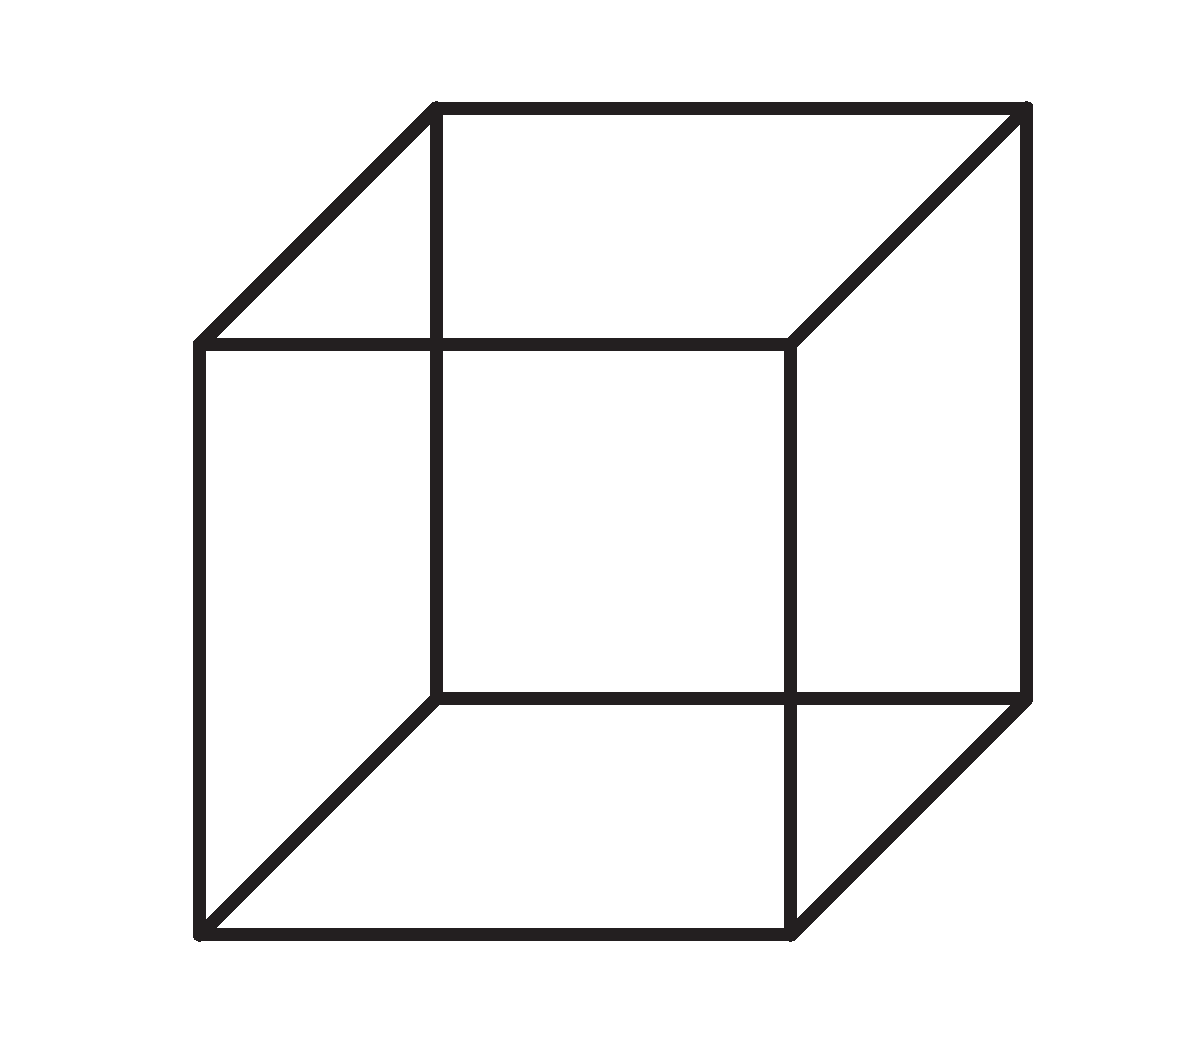
\includegraphics[width=30mm]{mask_rittai1.eps}
\end{center}
\end{figure}

\Subsection{2}

同じ三次元の立方体を,ずらした位置にもう一つ描きます.

\begin{figure}[h]
\begin{center}
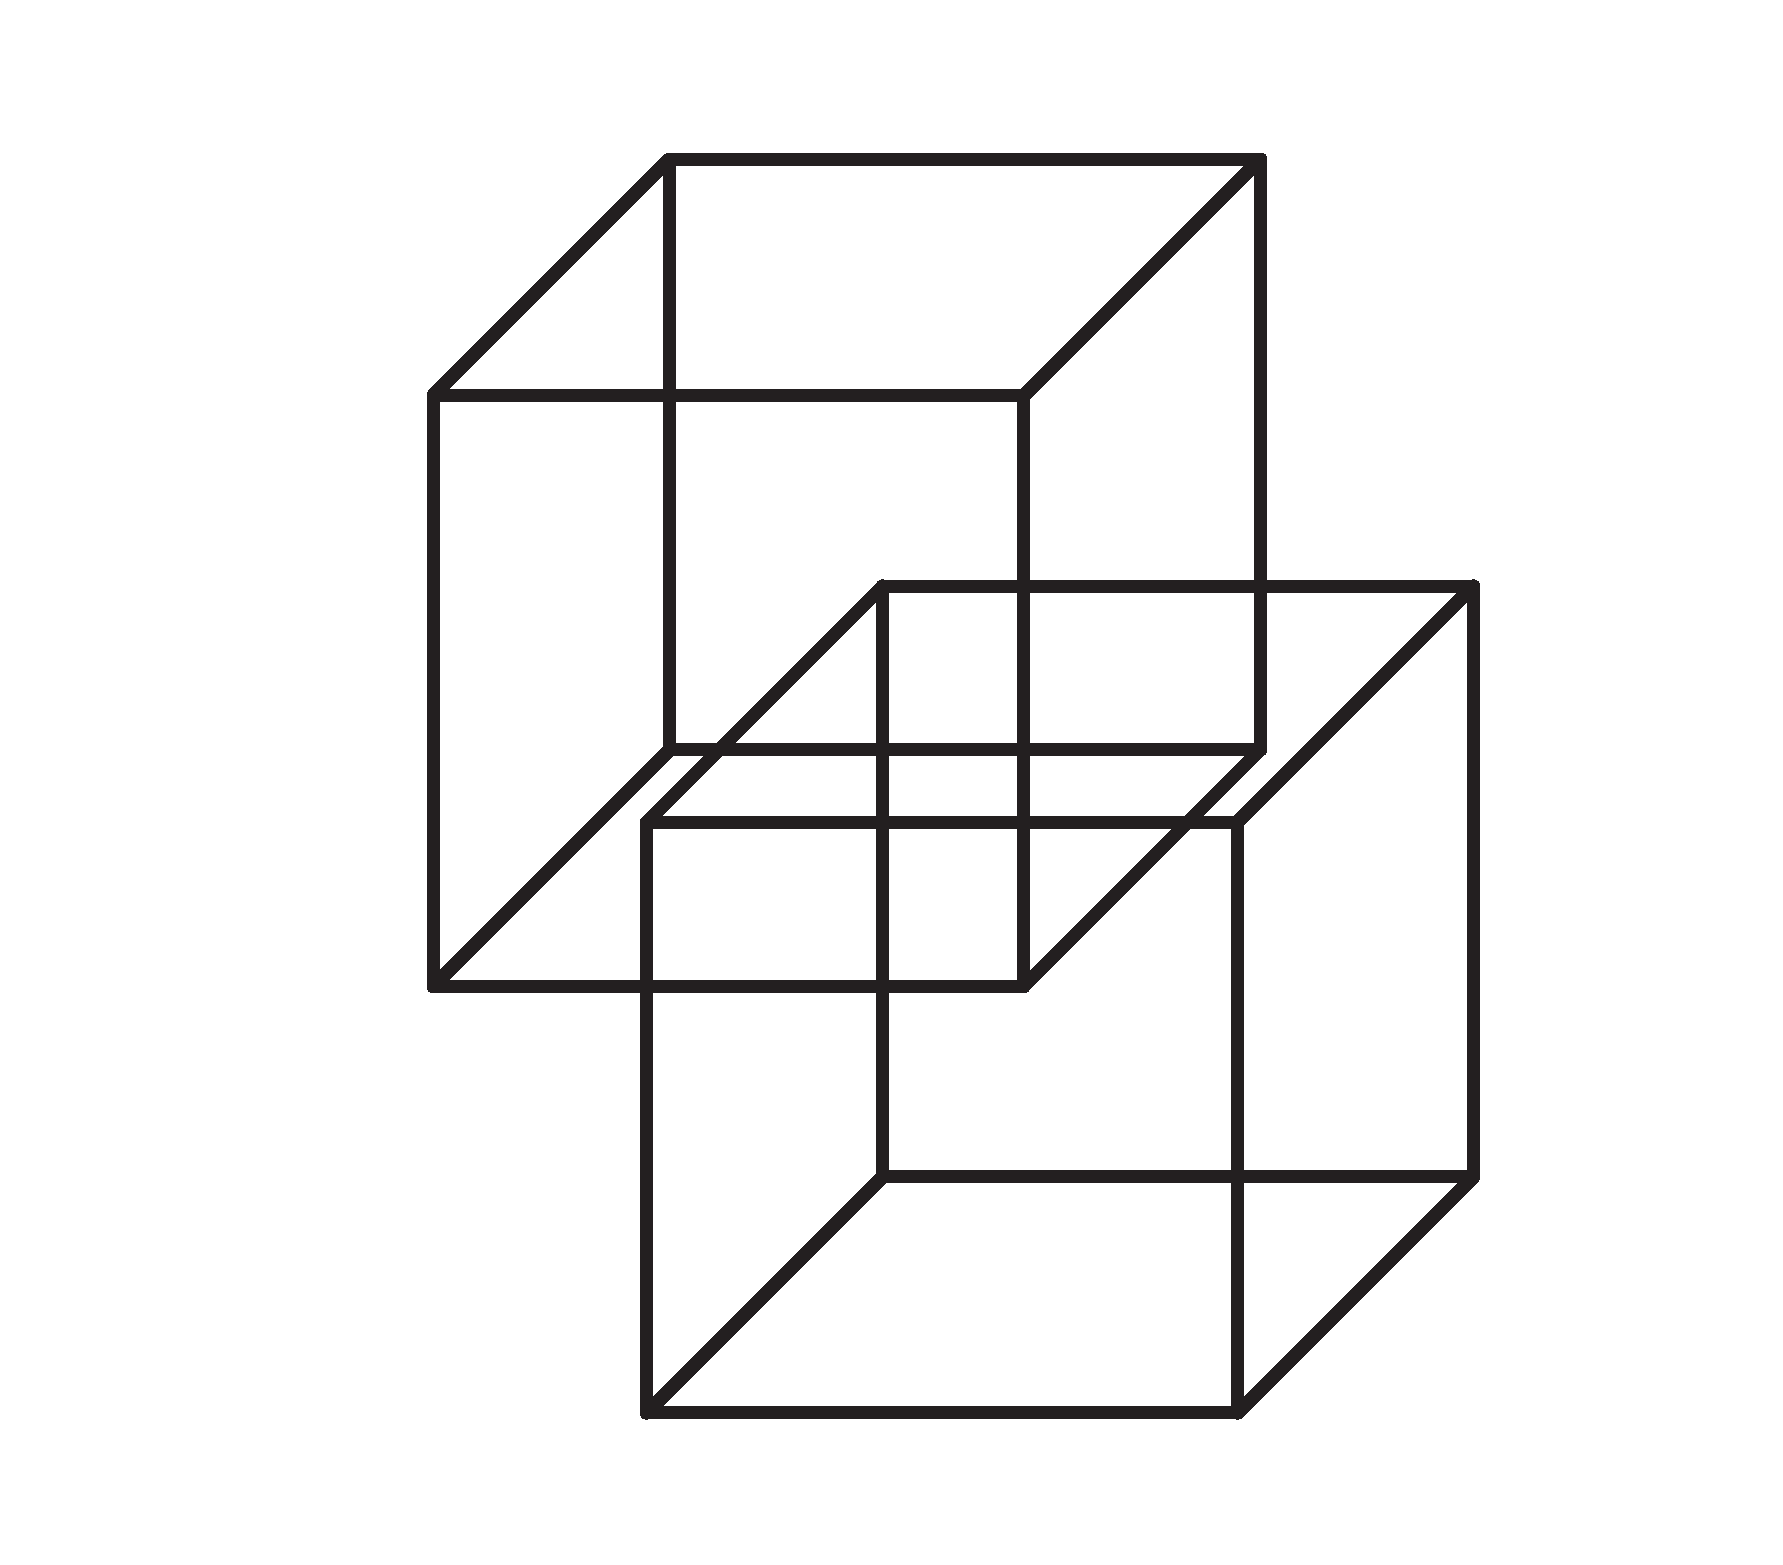
\includegraphics[width=48mm]{mask_rittai2.eps}
\end{center}
\end{figure}

\Subsection{3}

頂点を線分で結びます.

\begin{figure}[h]
\begin{center}
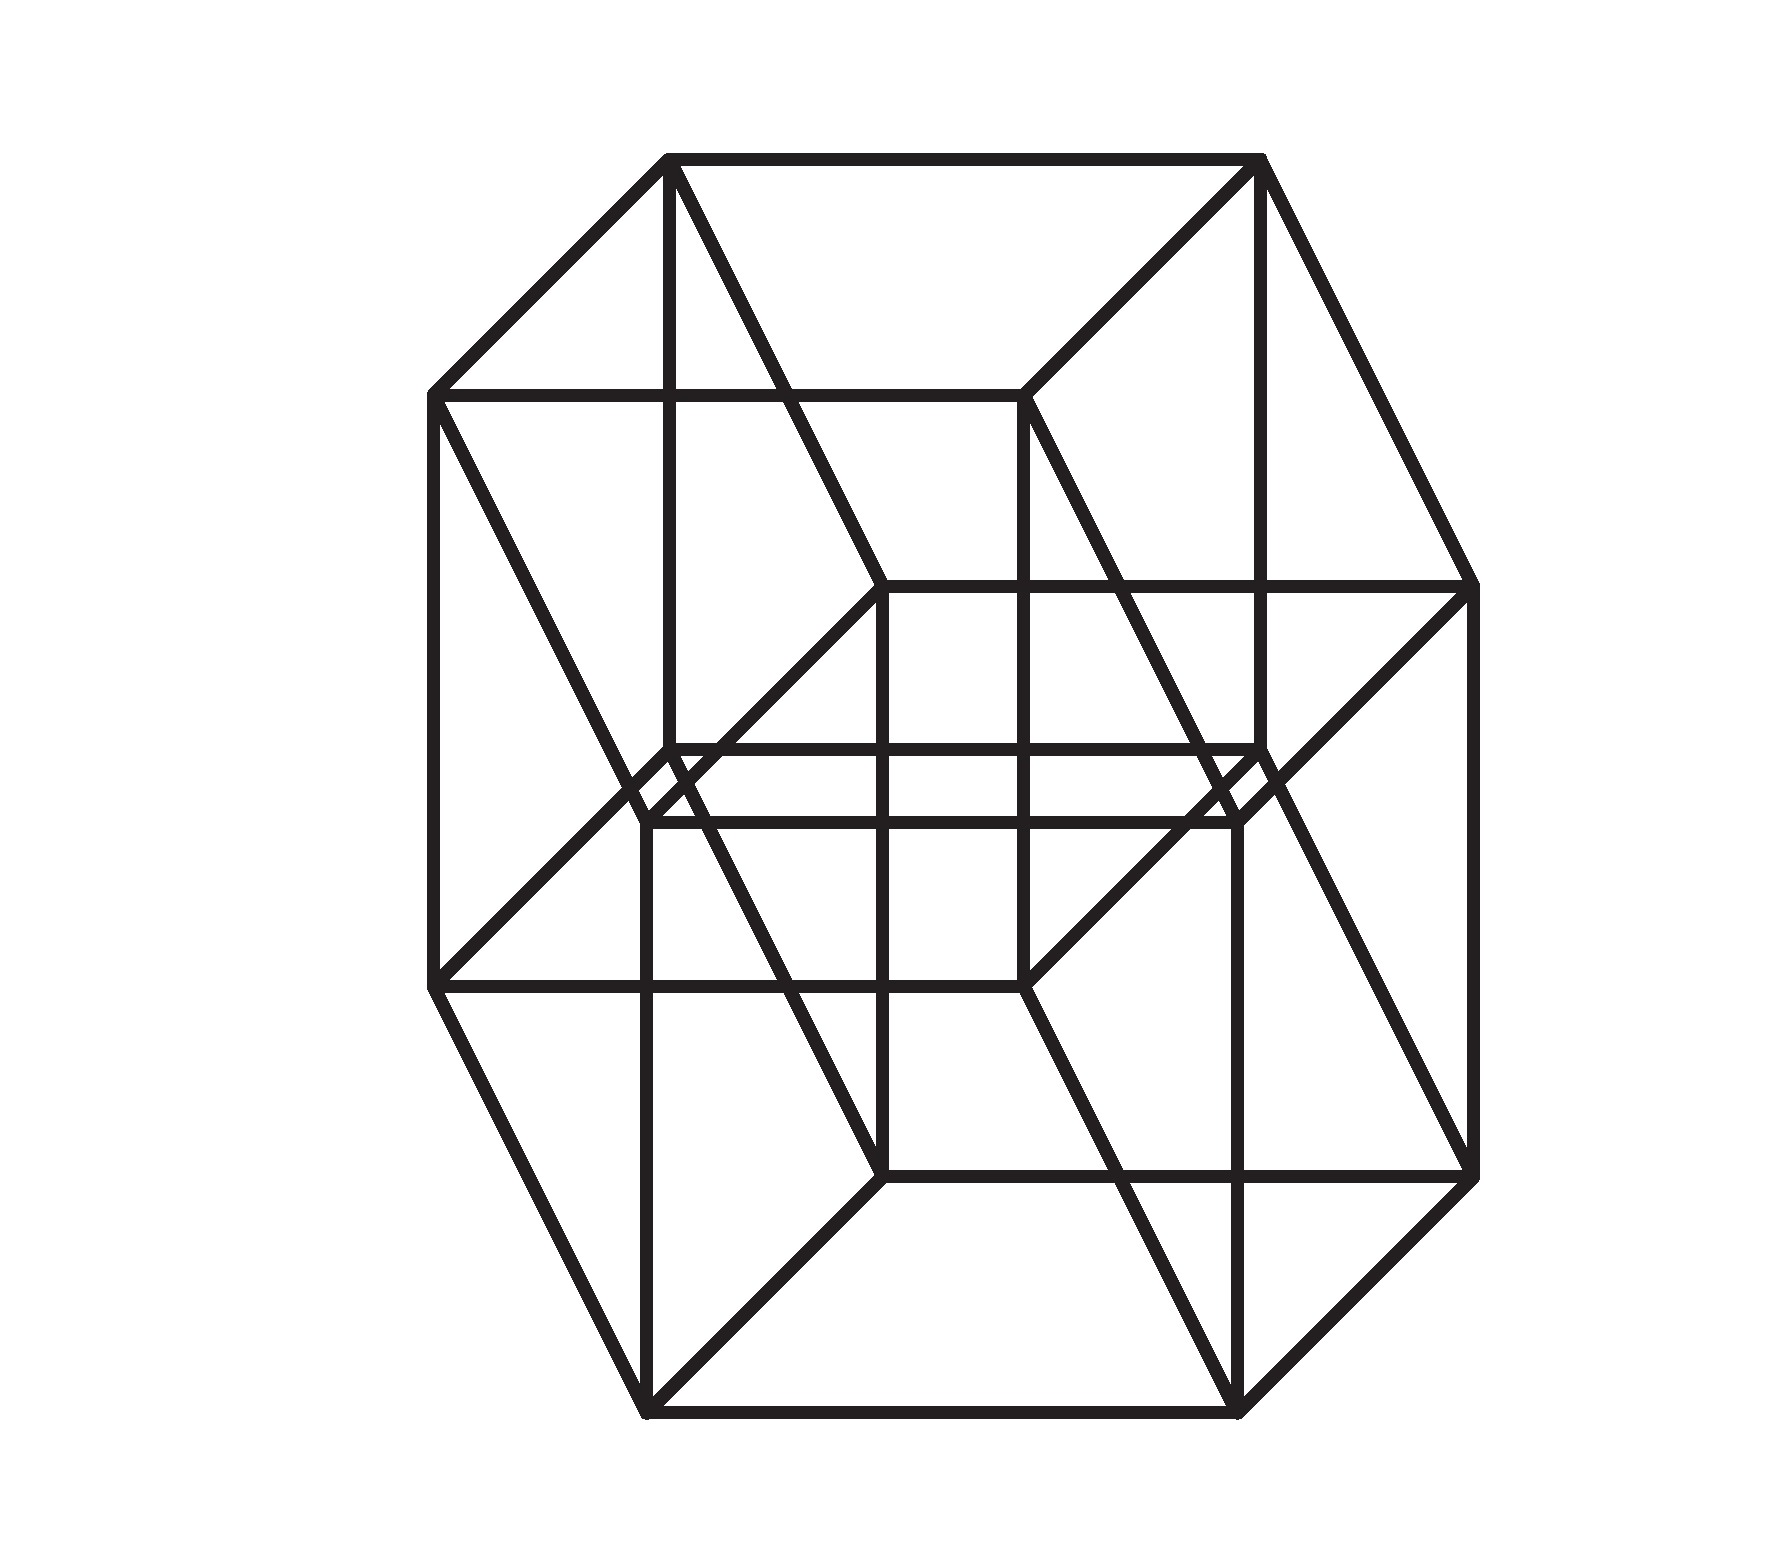
\includegraphics[width=48mm]{mask_rittai3.eps}
\end{center}
\end{figure}

これで完成です.

%追記します%

\end{document}

%\begin{thebibliography}{9}
%\item Hull, J. C. (2014), Options, Futures, and Other Derivatives, 9th edition (Upper Saddle River, NJ: Prentice Hall).
%\end{thebibliography}
